% This file was created by tikzplotlib v0.8.5.
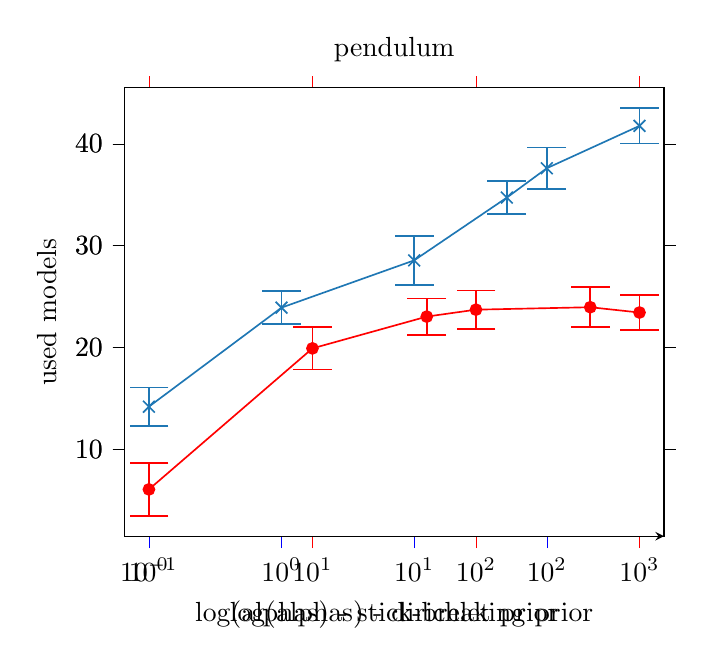
\begin{tikzpicture}

\definecolor{color0}{rgb}{0.12156862745098,0.466666666666667,0.705882352941177}

\begin{axis}[
log basis x={10},
tick align=outside,
tick pos=both,
title={pendulum},
x grid style={white!69.01960784313725!black},
xlabel={log(alphas) - stick-breaking prior},
xmin=0.707945784384138, xmax=1412.53754462275,
xmode=log,
xtick style={color=red},
xtick={0.01,0.1,1,10,100,1000,10000,100000},
xticklabels={\(\displaystyle {10^{-2}}\),\(\displaystyle {10^{-1}}\),\(\displaystyle {10^{0}}\),\(\displaystyle {10^{1}}\),\(\displaystyle {10^{2}}\),\(\displaystyle {10^{3}}\),\(\displaystyle {10^{4}}\),\(\displaystyle {10^{5}}\)},
y grid style={white!69.01960784313725!black},
ylabel={used models},
ymin=1.48903723098243, ymax=45.4868638620991,
ytick style={color=black}
]
\path [draw=red, semithick]
(axis cs:1,3.48893844148774)
--(axis cs:1,8.67106155851226);

\path [draw=red, semithick]
(axis cs:10,17.8430792022805)
--(axis cs:10,21.9969207977195);

\path [draw=red, semithick]
(axis cs:50,21.2628112086782)
--(axis cs:50,24.8171887913218);

\path [draw=red, semithick]
(axis cs:100,21.8327798220663)
--(axis cs:100,25.6072201779337);

\path [draw=red, semithick]
(axis cs:500,21.9906346199854)
--(axis cs:500,25.9293653800146);

\path [draw=red, semithick]
(axis cs:1000,21.7176759886711)
--(axis cs:1000,25.1623240113289);

\addplot [semithick, red, mark=-, mark size=7, mark options={solid}, only marks]
table {%
1 3.48893844148774
10 17.8430792022805
50 21.2628112086782
100 21.8327798220663
500 21.9906346199854
1000 21.7176759886711
};
\addplot [semithick, red, mark=-, mark size=7, mark options={solid}, only marks]
table {%
1 8.67106155851226
10 21.9969207977195
50 24.8171887913218
100 25.6072201779337
500 25.9293653800146
1000 25.1623240113289
};
\addplot [semithick, red, mark=*, mark size=2, mark options={solid}]
table {%
1 6.08
10 19.92
50 23.04
100 23.72
500 23.96
1000 23.44
};
\end{axis}

\begin{axis}[
axis x line=top,
log basis x={10},
tick align=outside,
tick pos=both,
x grid style={white!69.01960784313725!black},
xlabel={log(alphas) - dirichlet prior},
xmin=0.0653208007180445, xmax=765.452956031932,
xmode=log,
xtick style={color=blue},
xtick={0.001,0.01,0.1,1,10,100,1000,10000},
xticklabels={\(\displaystyle {10^{-3}}\),\(\displaystyle {10^{-2}}\),\(\displaystyle {10^{-1}}\),\(\displaystyle {10^{0}}\),\(\displaystyle {10^{1}}\),\(\displaystyle {10^{2}}\),\(\displaystyle {10^{3}}\),\(\displaystyle {10^{4}}\)},
y grid style={white!69.01960784313725!black},
ymin=1.48903723098243, ymax=45.4868638620991,
ytick style={color=black}
]
\path [draw=color0, semithick]
(axis cs:0.1,12.302633403899)
--(axis cs:0.1,16.097366596101);

\path [draw=color0, semithick]
(axis cs:1,22.2971629779919)
--(axis cs:1,25.5428370220081);

\path [draw=color0, semithick]
(axis cs:10,26.1586670368314)
--(axis cs:10,30.9613329631686);

\path [draw=color0, semithick]
(axis cs:50,33.0824408407633)
--(axis cs:50,36.3575591592367);

\path [draw=color0, semithick]
(axis cs:100,35.5800990123276)
--(axis cs:100,39.6199009876724);

\path [draw=color0, semithick]
(axis cs:500,40.0330373484062)
--(axis cs:500,43.4869626515938);

\addplot [semithick, color0, mark=-, mark size=7, mark options={solid}, only marks]
table {%
0.1 12.302633403899
1 22.2971629779919
10 26.1586670368314
50 33.0824408407633
100 35.5800990123276
500 40.0330373484062
};
\addplot [semithick, color0, mark=-, mark size=7, mark options={solid}, only marks]
table {%
0.1 16.097366596101
1 25.5428370220081
10 30.9613329631686
50 36.3575591592367
100 39.6199009876724
500 43.4869626515938
};
\addplot [semithick, color0, mark=x, mark size=3, mark options={solid}]
table {%
0.1 14.2
1 23.92
10 28.56
50 34.72
100 37.6
500 41.76
};
\end{axis}

\end{tikzpicture}
